    \documentclass[11pt]{article}
    %	options include 12pt or 11pt or 10pt
    %	classes include article, report, book, letter, thesis
    
    \title{HW4}
    \author{Shane Drafahl}
    \date{16 October ,2017}
    \usepackage{graphicx}
    \usepackage{epstopdf}
    \usepackage{graphics}

    \begin{document}
    \maketitle

     1. For union This means that the language accepted by the turring machine 
     is just a subset of a language that is already accepted. To biuld a turring machine
     I would just use double sided tape and would take a string from both languages that
     are unioned and put one on each side of the tape. I would then takes turns with 
     the algorithm on each perspective language on both sides of the tape. If both sides of the tape
     are accepted then the language is valid.

     $ \newline $
        Here is a small example of what the tape could look like. Where $ a_{n} $ is from one language
        and $ b_{n} $ is from another.
     $ \newline $

    \begin{figure}[!htb]
        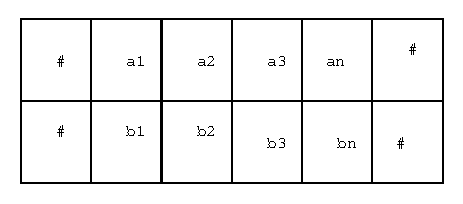
\includegraphics[scale=.7]{./turring.eps}
    \end{figure}

    $ \newline $

    For intersection I will still be using two sides of the tape but in this case if either side
    is accepted then the whole thing is accepted.

    $ \newline $

    \begin{figure}[!htb]
        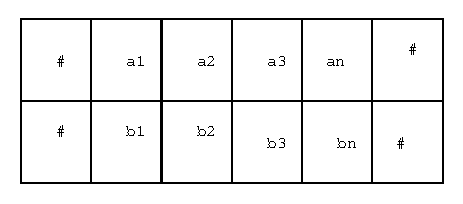
\includegraphics[scale=.7]{./turring.eps}
    \end{figure}

    $ \newline $

    For reversal I would simply copy the input from one side of the tape to the other in reverse
    order. I would then have the original accepts either side of the tape we know it is accepting.

    $ \newline $

    
    \end{document}